% From Qrrbrbirlbel
\documentclass[tikz,border=1cm]{standalone}
\usetikzlibrary{arrows.meta}
\tikzset{
        arrow shift factor/.initial=.5, % arrow shift option
        pics/arrow/.style={/tikz/sloped, /tikz/allow upside down,
        % /tikz/sloped用于让arrow与路径方向平行
        % /tikz/allow upside down关闭tikz自动调整side的功能
        setup code=\pgfarrowtotallength{#1}\pgftransformxshift{(\pgfkeysvalueof{/tikz/arrow shift factor})*\csname pgf@x\endcsname},%基于pgf提供的\pgfarrowdraw控制箭头
        code=\pgfarrowdraw{#1}}, 
        pics/arrow/.default=>
    } % handle设置默认值 .default
\begin{document}
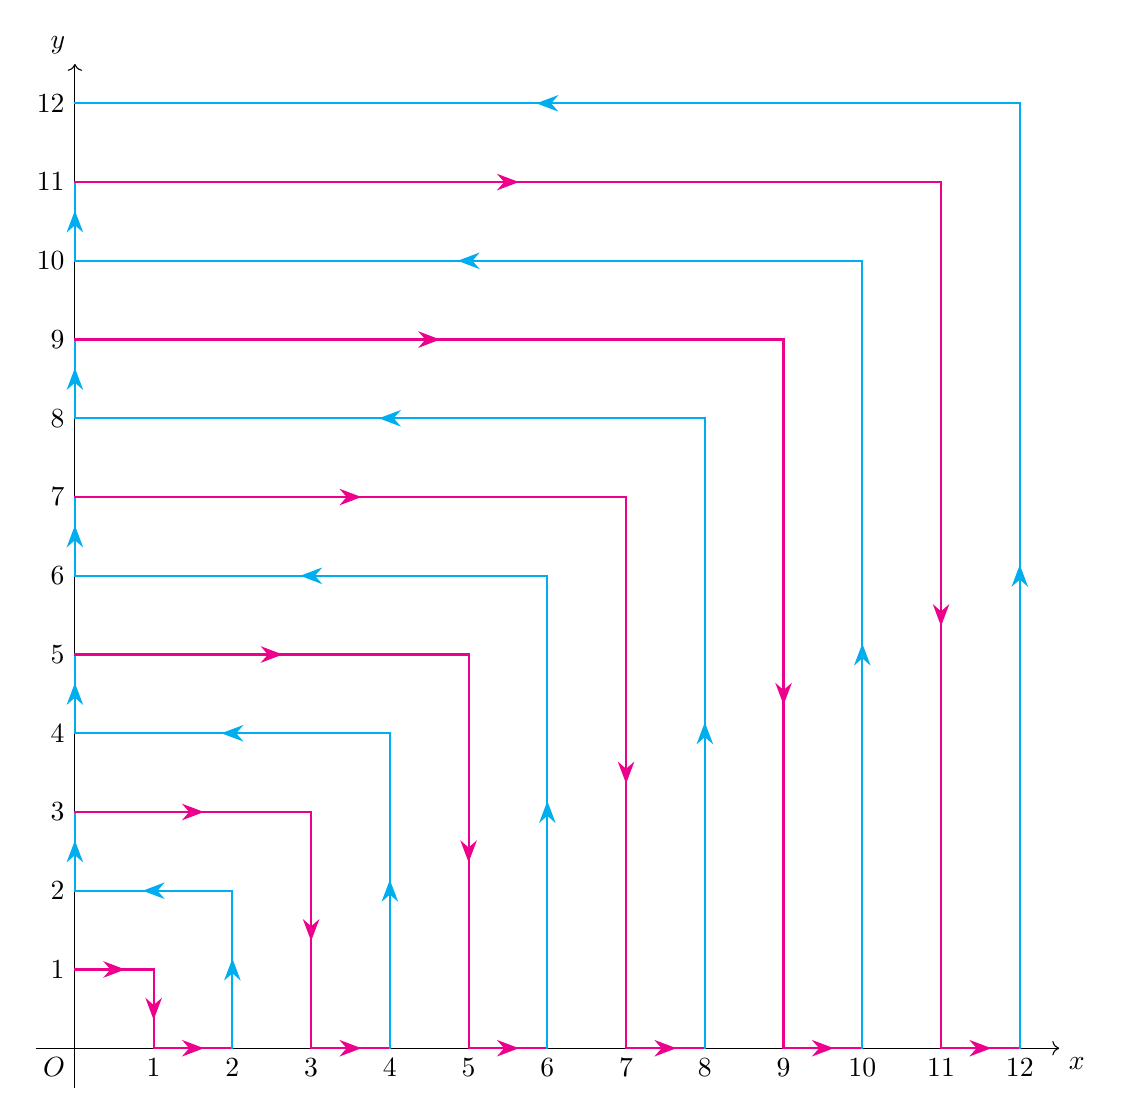
\begin{tikzpicture}[
  arrow node/.style=black,
  arrow odd/.style={
    magenta,% insert path用于在路径中插入对应符号
    % 神了!在绘制path的同时绘制坐标轴的标度
    insert path={(0,#1) node[arrow node, left ]{$#1$} to (#1,#1)
              to (#1,0) node[arrow node, below]{$#1$}
              \unless\ifnum#1=\NN to ++(right:1)\fi}},
              %使用\primitive \unless实现最后一段的优雅特判
  arrow even/.style={
    cyan,
    insert path={(#1,0) node[arrow node, below]{$#1$} to (#1,#1)
              to (0,#1) node[arrow node, left ]{$#1$}
              \unless\ifnum#1=\NN to ++(up:1)\fi}},
  arrow even or odd/.style={
    thick, line cap=rect,
    % every to句柄将自动合并在每个to(--)选项之后
    every to/.append style={edge node={pic[midway]{arrow={Stealth[scale=1.2]}}}}
  },
]
\newcommand*\NN{12}
\node[below left]{$O$};
% the 5mm specified with these shifts don't scale
% if you scale the xyz coordinate system, i.e.
% the axis always overshoot about 5mm
\draw[->] ([yshift=+-5mm]0,0) -- ([yshift=+5mm]   up:\NN) node[above left ]{$y$};
\draw[->] ([xshift=+-5mm]0,0) -- ([xshift=+5mm]right:\NN) node[below right]{$x$};
\foreach \i in {1, ..., \NN}
  \draw[
    arrow even or odd,
    arrow \ifodd\i\space odd\else even\fi=\i
  ];
\end{tikzpicture}
\end{document}